\documentclass{beamer}

\usepackage[utf8]{inputenc}
\usepackage{tikz}
\usepackage{graphicx}
\author{Jonathan Boidol, Rene Schoeffel, Yann Sp\"ori}
\title{HyPnOBrain}
\subtitle{your homology based HPO neural network predictor}
\date{\today}
%\usepackage{default}

\begin{document}

\begin{frame}
\maketitle
 
\end{frame}

\begin{frame}
  \frametitle{Homology based function prediction}
  General approach:
  \begin{itemize}
  	\item Search for annotated similar sequences\\with blast and hhblits (hits)
  	\item Build subgraph of HPO containing the found annotations
  	\item Calculate confidence for every annotation from some distance measure to the hits
  \end{itemize}

\end{frame}

\begin{frame}
	\frametitle{Preparations}
		\begin{itemize}
			\item Prepare databases for annotated sequences
			\item Represent HPO Graph in predictor
			\item Merge trees corresponding to hits
		\end{itemize}
		\begin{minipage}{0.2\textwidth}
			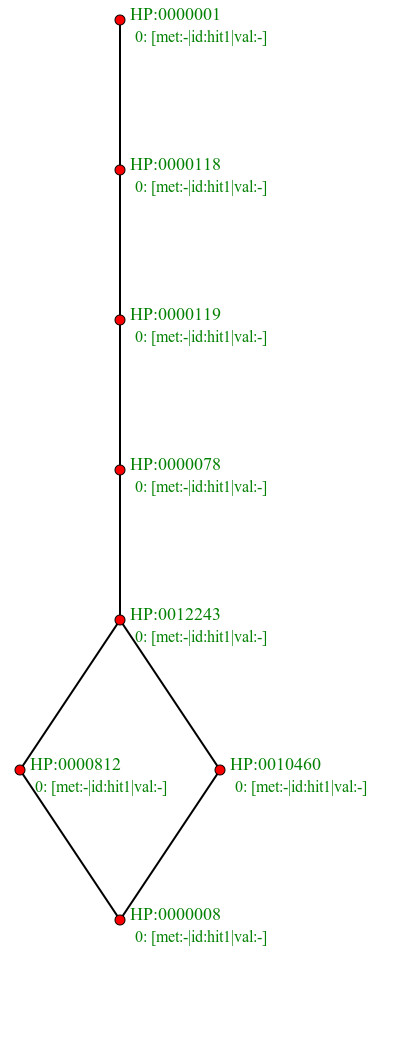
\includegraphics[width=\textwidth]{p1.jpg}	
		\end{minipage}$+$\hspace*{1em}
		\begin{minipage}{0.1\textwidth}
			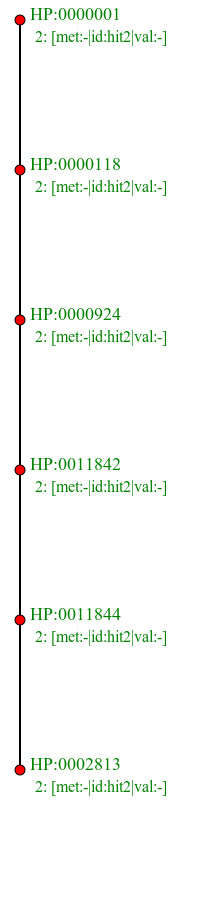
\includegraphics[width=\textwidth]{p2.jpg}\\
			\vspace*{1.0em}
		\end{minipage}$\Rightarrow$
		\begin{minipage}{0.3\textwidth}
		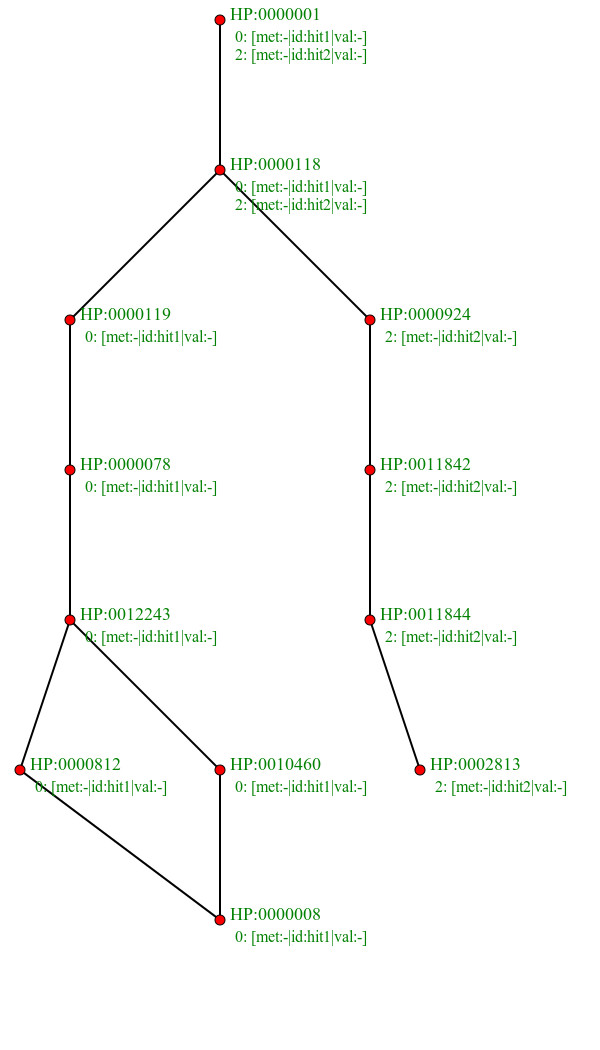
\includegraphics[width=\textwidth]{g.jpg}
		\end{minipage}
		
		
\end{frame}

\begin{frame}
	\frametitle{Features}
	\begin{itemize}
		\item use neural network to calculate confidence per node
		\item each node is assigned $x$ features derived from the merged tree
		\item[] \begin{itemize}
					\item number of hits
					\item min. E-value	
					\item avg. E-value \qquad[3, 0.0074, 0.45, 84, $\dots$]
					\item longest hit
					\item $\dots$ 
				\end{itemize}
				\item[] 
	\end{itemize}
\end{frame}

\begin{frame}
	\frametitle{Network architecture}
\begin{center}
	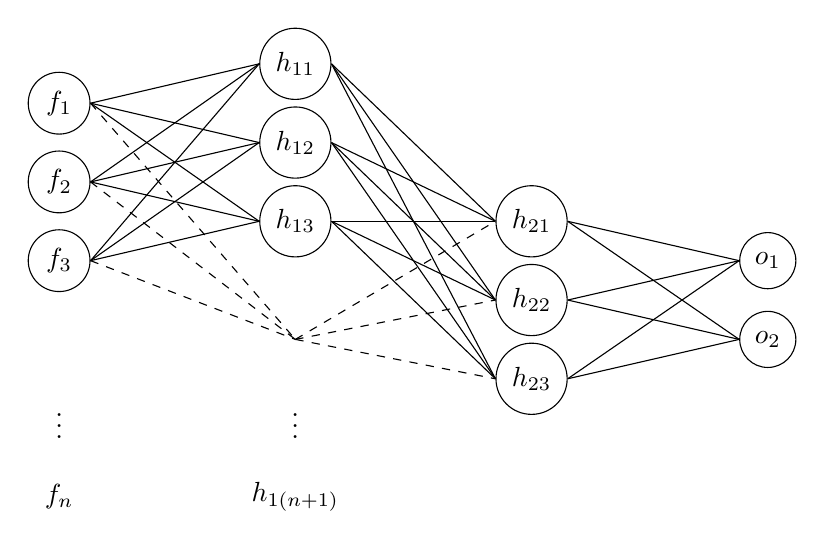
\begin{tikzpicture}[scale=1]
	
	%input nodes
	\node[draw, circle] (f1) at (0,4){$f_1$};
	\node[draw, circle] (f2) at (0,3){$f_2$};
	\node[draw, circle] (f3) at (0,2){$f_3$};
	\node[] at (0,0){$\vdots$};
	\node[] (fn) at (0,-1){$f_n$};
	
	%first hidden level
	\node[draw, circle] (h11) at (3,4.5){$h_{11}$};
	\node[draw, circle] (h12) at (3,3.5){$h_{12}$};
	\node[draw, circle] (h13) at (3,2.5){$h_{13}$};
	\node[] at (3,0){$\vdots$};
	\node[] (h1n) at (3,-1){$h_{1(n+1)}$};	
	
	%second hidden level
	\node[draw, circle] (h21) at (6,2.5){$h_{21}$};
	\node[draw, circle] (h22) at (6,1.5){$h_{22}$};
	\node[draw, circle] (h23) at (6,0.5){$h_{23}$};
	
	
	%output level
	\node[draw, circle] (o1) at (9,2){$o_{1}$};
	\node[draw, circle] (o2)at (9,1){$o_{2}$};
	
	\draw (f1.east) -- (h11.west);
	\draw (f1.east) -- (h12.west);
	\draw (f1.east) -- (h13.west);
	\draw (f1.east)[dashed] -- (3,1);

	\draw (f2.east) -- (h11.west);
	\draw (f2.east) -- (h12.west);
	\draw (f2.east) -- (h13.west);
	\draw (f2.east)[dashed] -- (3,1);

	\draw (f3.east) -- (h11.west);
	\draw (f3.east) -- (h12.west);
	\draw (f3.east) -- (h13.west);
	\draw (f3.east)[dashed] -- (3,1);
	
	\draw (h11.east) -- (h21.west);
	\draw (h11.east) -- (h22.west);
	\draw (h11.east) -- (h23.west);

	\draw (h12.east) -- (h21.west);
	\draw (h12.east) -- (h22.west);
	\draw (h12.east) -- (h23.west);

	\draw (h13.east) -- (h21.west);
	\draw (h13.east) -- (h22.west);
	\draw (h13.east) -- (h23.west);

	\draw (3,1)[dashed] -- (h21.west);
	\draw (3,1)[dashed] -- (h22.west);
	\draw (3,1)[dashed] -- (h23.west);
	
	\draw (h21.east) -- (o1.west);
	\draw (h21.east) -- (o2.west);
	
	\draw (h22.east) -- (o1.west);
	\draw (h22.east) -- (o2.west);
	
	\draw (h23.east) -- (o1.west);
	\draw (h23.east) -- (o2.west);
	
	\end{tikzpicture}
\end{center}
	\hfill\\
	\begin{itemize}
		\item fully connected net with two hidden layers
		\item two output nodes trained for the two possible predictions
		\item difference of predictions as confidence
	\end{itemize}	
\end{frame}

\begin{frame}
	\frametitle{Validation}
	
	\begin{itemize}
		\item Inspection of the dataset shows: Most sequences have pairwise similarity $< 80\%$
		\item[] $\Rightarrow$ reduce set at $80\%$-level to remove highly similar clusters
		\item Crossvalidate over reduced set but allow non-reduced trainingset for similarity search during testing
		\item Calculate precision and recall per test sequence and average over all sequences
	\end{itemize}
\end{frame}

\begin{frame}
	\frametitle{Results}
	Pre-Rec-Curve here\\
	\hfill\\
	\hfill\\
	\hfill\\
	\begin{itemize}
		\item F-measure $yy$ (at confidence level $x$)
		\item Precision (at same confidence level $x$)
		\item Recall (at same confidence level $x$)
	\end{itemize}		
	
\end{frame}


\end{document}
